% !TeX program = lualatex
\documentclass[a4paper,11pt]{ltjsarticle}

\usepackage[margin=24mm]{geometry}
\usepackage{amsmath,amssymb,mathtools}
\usepackage{tikz}
\usetikzlibrary{calc,angles,quotes}
\usepackage{hyperref}

\hypersetup{
  colorlinks=true,
  linkcolor=blue,
  urlcolor=blue
}

\title{三角比を使わないヘロンの公式の図形的証明}
\author{}
\date{}

\usepackage{tikz}

\newcommand{\marunum}[1]{%
  \tikz[baseline=(X.base)]{
    \node[
      circle,
      fill=black,
      text=white,
      font=\bfseries\small,
      inner sep=0pt,
      minimum size=1em
    ] (X) {#1};
  }%
}

\newcommand{\Area}{\mathcal{A}}
 
\begin{document}
\begin{center}
{\bf \large 三角比を使わないヘロンの公式の証明}
\end{center}

三角形 ${\rm ABC}$ の辺の長さを $a={\rm BC}$,\, $b={\rm CA}$,\, $c={\rm AB}$とするとき, 周長 (pelimeter) は$p=a+b+c$であるが, その半分を半周長 (semipelimeter) といって$s=p/2$で定義する. このとき, $\triangle{\rm ABC}$の面積が
$\boxed{[{\rm ABC}]=\sqrt{s(s-a)(s-b)(s-c)}}$で計算できるという定理があり, これはヘロンの公式と呼ばれている. 正弦定理や余弦定理を使わず, 三角形の相似と{\bf 内心}と{\bf 傍心}の定義だけで証明してみよう. 

①三角形の角の二等分線３本は１点で交わり, 内接円の中心となる（これを内心とよび下図で$\rm I$と表記する）, ②三角形の２つの外角の二等分線の交点（傍心）を中心とする外接円（これを傍接円とよぶ）を描ける,  という２つの有名な事実を認めることにする.  下図のように点$\rm A$の辺$\rm BC$に対する反対側の傍心を${\rm I}_a$で表記する.

\begin{center}
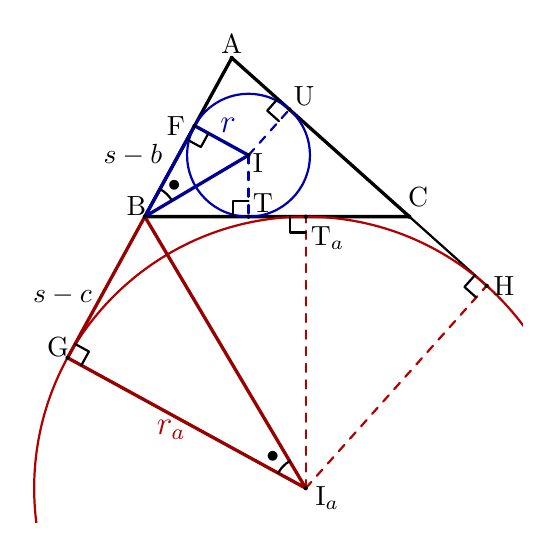
\begin{tikzpicture}[scale=0.48,
  line cap=round,
  line join=round,
  every node/.style={font=\small}]

  % 実際の座標（計算済み）
  \coordinate (A)  at ( 2.300, 4.200);
  \coordinate (B)  at ( 0.000, 0.000);
  \coordinate (C)  at ( 7.000, 0.000);
  \coordinate (I)  at ( 2.743, 1.625);
  \coordinate (Ia) at ( 4.257,-7.185);
  \coordinate (F)  at ( 1.317, 2.406);
  \coordinate (G)  at (-2.045,-3.734);
  \coordinate (T)  at ( 2.743, 0.000);
  \coordinate (Ta) at ( 4.257, 0.000);

  % 追加：AC 上の内接円接点 U，AC 延長上の A-傍接円接点 H
  \coordinate (U)  at ( 3.826, 2.837);
  \coordinate (H)  at ( 9.045,-1.827);

  % 描画範囲を制限（傍接円の下半分は省略）
  \clip (-3.1,-8.1) rectangle (10.0,5.0);

  % 三角形と辺の延長
  \draw[very thick] (A)--(B)--(C)--cycle;
  %\draw[thick] (A)--($(B)!1.62!(A)$);
% \draw[thick] ($(B)!1.52!(A)$)--(B);

  % AC の延長（H を見せるため）
  %\draw[thick] (A)--($(C)!1.45!(A)$);
  \draw[thick] (C)--($(A)!1.45!(C)$);

  % 内接円（半径 1.625）
  \draw[blue!70!black,thick] (I) circle[radius=1.625];

  % A傍接円（半径 7.185, 必要な部分だけ見える）
  \draw[red!70!black,thick] (Ia) circle[radius=7.185];

  % 半径および相似に使う線分
  \draw[blue!70!black,dashed,thick] (I)--(F);
  \draw[blue!70!black,dashed,thick] (I)--(T);
  \draw[blue!70!black,dashed,thick] (I)--(U);

  \draw[red!70!black,dashed,thick] (Ia)--(G);
  \draw[red!70!black,dashed,thick] (Ia)--(Ta);
  \draw[red!70!black,dashed,thick] (Ia)--(H);

  \draw[blue!60!black,very thick] (B)--(F)--(I)--cycle;
  \draw[red!60!black,very thick] (B)--(G)--(Ia)--cycle;

  % 直角記号
  \pic[draw,angle radius=2mm,thick] {right angle = B--F--I};
  \pic[draw,angle radius=2mm,thick] {right angle = B--G--Ia};
  \pic[draw,angle radius=2mm,thick] {right angle = B--T--I};
  \pic[draw,angle radius=2mm,thick] {right angle = B--Ta--Ia};
  \pic[draw,angle radius=2mm,thick] {right angle = A--U--I};
  \pic[draw,angle radius=2mm,thick] {right angle = A--H--Ia};

  % 角 B/2
\pic[draw,thick,angle radius=4mm,angle eccentricity=1.35,
     "$\bullet$"] {angle = I--B--F};
  \pic[draw,  thick,angle radius=4mm,angle eccentricity=1.45,
       "$\bullet$"] {angle = B--Ia--G};

  % 点
\fill (A) circle(1.6pt)
  node[above,yshift=-2pt,font=\normalsize] {$\mathrm{A}$};
\fill (B) circle(1.6pt)
  node[above left,xshift=4pt,yshift=-3pt,font=\normalsize] {$\mathrm{B}$};
\fill (C) circle(1.6pt)
  node[above right,xshift=-4pt,font=\normalsize] {$\mathrm{C}$};
\fill (I) circle(1.6pt)
  node[below right,xshift=-2pt,yshift=4pt,font=\normalsize] {$\mathrm{I}$};
\fill (Ia) circle(1.6pt)
  node[below right,xshift=0pt,yshift=4pt,font=\normalsize] {$\mathrm{I}_a$};

\fill (F) circle(1.6pt)
  node[left,xshift=0pt,font=\normalsize] {$\mathrm{F}$};
\fill (G) circle(1.6pt)
  node[above left,xshift=4pt,yshift=-3pt,font=\normalsize] {$\mathrm{G}$};
\fill (T) circle(1.6pt)
  node[above right,xshift=-2pt,yshift=-2pt,font=\normalsize] {$\mathrm{T}$};
\fill (Ta) circle(1.6pt)
  node[below right,xshift=-1.7pt,yshift=-0pt,font=\normalsize] {$\mathrm{T}_a$};

\fill (U) circle(1.6pt)
  node[above right,xshift=-2pt,yshift=-2pt,font=\normalsize] {$\mathrm{U}$};
\fill (H) circle(1.6pt)
  node[right,xshift=-1pt,font=\normalsize] {$\mathrm{H}$};

  % 半径・接線長
\node[blue!70!black,font=\large]
  at ($(I)!0.52!(F)+(0.2,0.38)$) {$r$};

\node[red!70!black,font=\large]
  at ($(Ia)!0.53!(G)+(-0.22,-0.28)$) {$r_a$};

\node[font=\normalsize]
  at ($(B)!0.52!(F)+(-1,+0.38)$) {$s-b$};

\node[font=\normalsize]
  at ($(B)!0.48!(G)+(-1.2,-0.30)$) {$s-c$};

\end{tikzpicture}
\end{center}


ヘロンの公式は以下で証明する\marunum{1}～\marunum{5}による.  以下では,  $r$ を内接円の半径とし, 傍接円の${\rm I}_a$ の半径を$r_a$とおく.

\marunum{1}$まず\boxed{{\rm BF}=s-b}$を確認する. これは中学数学の問題である. ①より${\rm BF}=x={\rm BT}$でおけば, ${\rm TC}=a-x={\rm CU}$になるから, ${\rm AU}=b-(a-x)={\rm AF}$となる. ${\rm AF}=c-x$なので$2x=a+c-b$とわかる. これは$=2s-2b$なので$x=s-b$がわかった. 


\marunum{2}上と似た証明であるが, $\boxed{{\rm BG}=s-c}$は少し難しい. 

(i) ②より${\rm BG=BT}_a=y$, ${\rm T}_a{\rm C=CH}=z$とおけるので, 足せば$y+z=a$.


(ii) 直角三角形${\rm AGI}_a$と${\rm AHI}_a$は底辺を$r_a$, 斜辺を共通として合同であるから$\rm AG=AH$となり, $y$と$z$の差は
$y-z=b-c$になる.


(i)と(ii)より$2y=a+b-c=2s-2c$となり, $y=s-c$になる. 





\marunum{3}公式 $\boxed{{\rm [ABC]}=rs}$を確認しよう.  これも中学数学の問題である. $[\rm ABC]= [\rm AIB]+[\rm BIC]+[\rm CIA]$であるので, 高さを$r$として, $= \frac12 cr+\frac12 ar+\frac12 br= \frac12(a+b+c)r=rs  $と計算できる.

\marunum{4} $\boxed{[{\rm ABC}]=r_a(s-a)}$がなりたつ.  これは$[{\rm ABC}]= {[ {\rm ABI}_a]+[ {\rm ACI}_a]-[{\rm BCI}_a]}$であるため, $= \frac12cr_a+\frac12br_a-\frac12ar_a= \frac12(b+c-a)r_a= r_a(s-a)$で計算できる.



\marunum{5}最後に, 公式$ \boxed{rr_a=(s-b)(s-c)}$を示そう. $\angle {\rm BI}_a{\rm G}={\rm B}/2$であるため, ${\rm  \triangle BFI}$と${\rm \triangle I}_a{\rm GB}$は相似.  従って${\rm BF}:{r_a}={r}:{\rm BG}$により${\rm  BF\cdot BG}=rr_a$. \marunum{1}と\marunum{2}を代入すれば$rr_a=(s-b)(s-c)$.


以上の\marunum{3}, \marunum{4}, \marunum{5}を組み合わせれば, 
\[
 \boxed{[{\rm ABC}]^2=s(s-a)(s-b)(s-c)}
\]
が得られる. ■







\end{document}
